\chapter{Modelo de datos}
En este capítulo se describe el modelo de datos utilizado para persistir el sistema desarrollado.

\section{Modelo E-R}
%DietNow utiliza el software Google Firebase para almacenar toda la información necesaria para su correcto funcionamiento. Google Firebase y su sistema Realtime Database proporcionan una base de datos organizada en forma de árbol JSON, es decir, utilizan un sistema noSQL \cite{Techighness} que ofrece un gran número de ventajas técnicas y de flexibilidad que, unido a las ventajas de Realtime Database, como por ejemplo la sincronización en tiempo real y el SDK de la plataforma, proporcionan una base sólida sobre la cual se asienta el \textit{backend} de la aplicación.%

%Toda la información almacenada por DietNow se organiza en las siguientes tablas: Usuarios, Dietas, Alimentos, Comentarios, Pasos, Pesos e Historial de dietas. Las entradas de dichas tablas tendrán identificadores únicos generados automáticamente por el sistema gestor de base de datos Firebase a excepción de la tabla de alimentos que contendrá como identificador el código de barras si el alimento se recoge de la API OpenFoodFacts \cite{open_food_facts} o identificadores alfanuméricos que identifican a los alimentos que han sido dados de alta manualmente.%

%Los archivos se almacenan mediante Firebase Storage que proporciona cargas y descargas seguras de archivos para aplicaciones Firebase, sin importar la calidad de la red. Se puede utilizar para almacenar imágenes, audio, vídeo, o cualquier otro contenido generado por el usuario.

Como se aprecia en la figura \ref{fig:diagrama_e_r}, el diagrama entidad relación representa las distintas entidades y atributos que componen el sistema. Toda la información almacenada se representa mediante las siguientes colección de documentos: Usuarios, Dietas, Alimentos, Comentarios, Pasos, Pesos e Historial de dietas.

El sistema guarda información de los usuarios, los cuales pueden crear dietas. A su vez, la dieta guarda información sobre la cantidad de cada alimento que tiene que ingerir el deportista. Para poder llevar a cabo la funcionalidad principal de la aplicación, el usuario puede crear dietas que posteriormente pueden ser seguidas por otros usuarios. Para realizar el seguimiento de la dieta del usuario, se crea un historial donde se almacena por cada día la cantidad consumida de cada alimento. El usuario además puede ver y publicar comentarios sobre la dieta que sigue actualmente.\\
La aplicación cuenta también con distintos usuarios administradores encargados de supervisar los diferentes usuarios y dietas del sistema.

\begin{figure}[H]
    \centering
    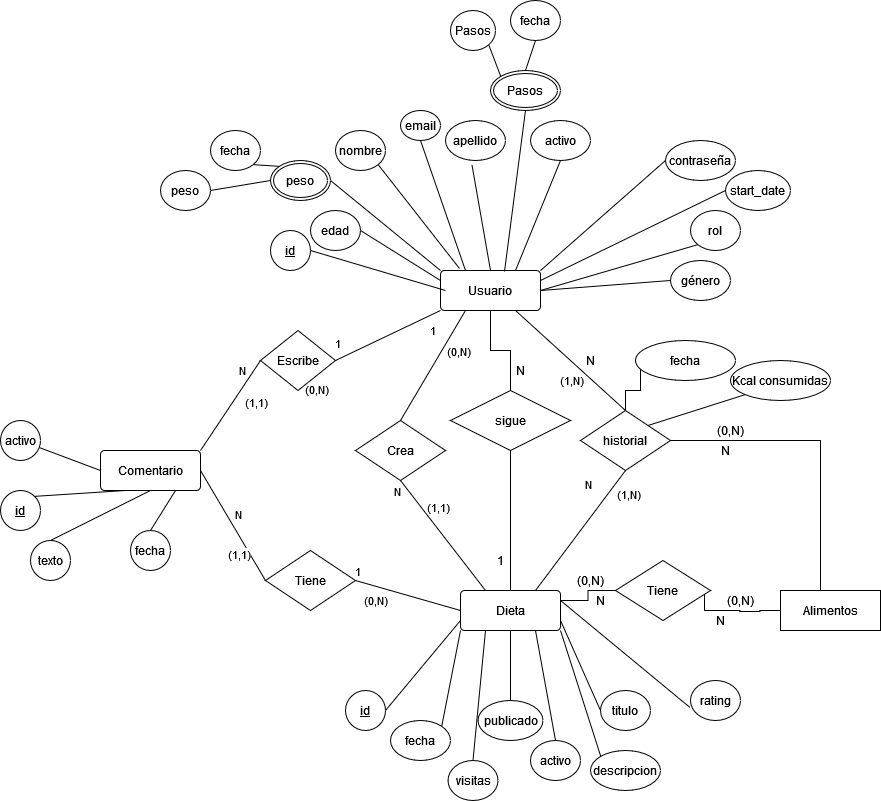
\includegraphics[width=\textwidth]{Images/Capitulo5/bbdd.drawio.png}
    \caption{Diagrama Entidad Relación}
    \label{fig:diagrama_e_r}
\end{figure}

\section{Implementación de la base de datos}
%%%%%%%%%%%%%%%%%%%%%%%%%%%%%%%
%%%%%TABLA DE USUARIOS%%%%%%%%%
%%%%%%%%%%%%%%%%%%%%%%%%%%%%%%%
El modelo E-R se implementa mediante una base de datos de tipo NoSQL, donde los datos son almacenados como documentos JSON \cite{json}. A continuación, se describen cada uno de ellos.

\subsection{Colección de documentos de usuarios}
Esta colección de documentos contiene la información de cada usuario registrado en la aplicación (ver figura \ref{fig:tabla_user}).

Concretamente contiene una lista de identificadores únicos para cada usuario y para cada identificador están asociados los siguientes campos:

\begin{itemize}
\item \textbf{Identificador de usuario} generado automáticamente por Firebase.
    \begin{itemize}
        \item \textbf{Active}: booleano que indica si la cuenta del usuario está activa o no. Todos los usuarios registrados tienen el valor \texttt{True} y los usuarios que se han dado de baja tienen este campo con el valor a \texttt{False}.
        \item \textbf{Age}: campo numérico que indica la edad del usuario.
        \item \textbf{Diet}: contiene el ID de la dieta que está siguiendo actualmente el usuario.
        \item \textbf{Email}: almacena el correo electrónico del usuario, necesario para que éste pueda iniciar sesión en la aplicación, además de ser un canal de comunicación en caso de que sea necesario enviar una notificación al usuario.
        \item \textbf{Gender}: campo que almacena el género del usuario, los valores posibles son \texttt{MALE} (Hombre), \texttt{FEMALE} (Mujer), \texttt{NO\_GENRE} (Prefiero no especificar).
        \item \textbf{Height}: campo que guarda la altura del usuario.
        \item \textbf{Lastname}: apellidos del usuario.
        \item \textbf{Name}: nombre del usuario.
        \item \textbf{Password}: campo que guarda encriptada la contraseña del usuario (mediante \texttt{jBcrypt} \cite{jbcrypt}). Cuando el usuario desea cambiar su contraseña, se comprueba este valor junto con la la nueva contraseña cifrada para verificar que es distinta y proceder al cambio de la misma.
        \item \textbf{Role}: campo que almacena el rol del usuario, los valores posibles son USER y ADMIN.
        \item \textbf{Start date}: campo que guarda la fecha en la que se dio de alta el usuario en la aplicación.
        \end{itemize}
\end{itemize}


%FOTO DE LA TABLA%
\begin{figure}[H]
    \centering
    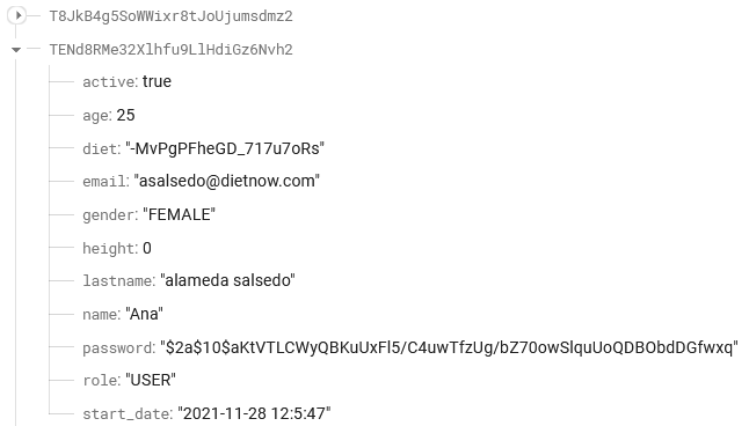
\includegraphics[width=0.9\textwidth]{Images/Capitulo5/Tabla_users.png}
    \caption{Colección de documentos de los usuarios}
    \label{fig:tabla_user}
\end{figure}
\newpage


%%%%%%%%%%%%%%%%%%%%%
%%%TABLA DE DIETAS%%%
%%%%%%%%%%%%%%%%%%%%%

\subsection{Colección de documentos de dietas}
Esta colección de documentos contiene la información de cada dieta registrado en la aplicación (ver figura \ref{fig:tabla_diet}).

Concretamente la colección de documentos de dietas contiene una lista de identificadores únicos para cada dieta registrada en la aplicación. Para cada identificador están asociados los siguientes campos:

\begin{itemize}
\item \textbf{Identificador de la dieta} generado automáticamente por Firebase.
    \begin{itemize}
        \item \textbf{Active}: booleano que indica si la dieta está activa o no. Todas las dietas creadas por defecto tienen el valor \texttt{True} y si el usuario autor de una dieta la ha dado de baja este campo tendrá el valor  \texttt{False}.
        \item \textbf{Aliments}: campo que almacena una lista de alimentos, la estructura utilizada es una lista de identificadores de alimentos y dentro de cada identificador, la información del alimento en cuestión con los siguientes campos:
        \begin{itemize}
            \item \textbf{Active}: booleano que indica si el alimento está activo o no.
            \item \textbf{Grams}: los gramos que tiene el alimento.
            \item \textbf{Kcal}: las kilocalorías del alimento.
            \item \textbf{Name}: nombre del alimento.
        \end{itemize}
        
        \item \textbf{Date}: la fecha en la que se creó la dieta.
        \item \textbf{Description}: campo que guarda la descripción que le ha puesto el autor a la dieta.
        \item \textbf{Id}: campo que almacena el identificador de la dieta
        \item \textbf{Published}: booleano que indica si la dieta está publicada o no. \texttt{True} indica que la dieta está publicada y la puede ver cualquier usuario de la aplicación y \texttt{False} indica que la dieta no está publicada y solo la puede ver su autor.
        \item \textbf{Rating}: campo que almacena una lista de usuarios que han valorado la aplicación. Guarda el id de los usuarios en un hashmap donde la clave es el id y el valor es un booleano, si el valor es \texttt{True} significa que el usuario ha dado \textit{like} a la dieta, si el valor es \texttt{False} significa que el usuario ha dado \textit{dislike}.
        \item \textbf{Title}: título de la dieta.
        \item \textbf{User}: campo que almacena el identificador del usuario que ha creado la dieta.
        \item \textbf{Visits}: campo que almacena una lista de usuarios que han visitado la aplicación. Guarda el id de los usuarios en un hashmap donde la clave es el id y el valor es un booleano a \texttt{True}.
    \end{itemize}
\end{itemize}



%FOTO DE LA TABLA%
\begin{figure}[H]
    \centering
    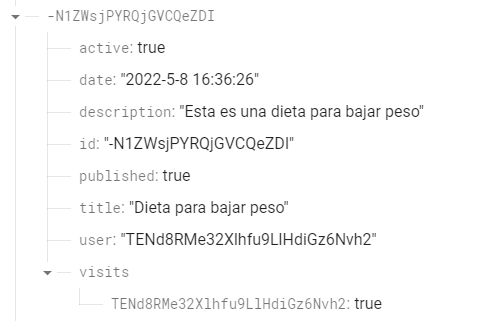
\includegraphics[width=0.9\textwidth]{Images/Capitulo5/tabla_diet.png}
    \caption{Entrada de la colección de documentos de dietas}
    \label{fig:tabla_diet}
\end{figure}

%%%%%%%%%%%%%%%%%%%%%
%%%TABLA DE ALIMENTOS
%%%%%%%%%%%%%%%%%%%%%

\subsection{Colección de documentos de alimentos}
Esta colección de documentos contiene la información de cada alimento registrado en la aplicación (ver figura \ref{fig:tabla_aliments}).

Concretamente contiene una lista de identificadores únicos. Existen 2 formatos de identificador para esta colección de documentos, los identificadores numéricos, el código de barras que identifica a cada alimento y los identificadores alfanuméricos que identifican a los alimentos que han sido dados de alta manualmente por el usuario. Independientemente del tipo de identificador, cada alimento registrado en la aplicación están asociados los siguientes campos:

\begin{itemize}
\item \textbf{Identificador del alimento} generado por la API Open Food Facts o manualmente.
    \begin{itemize}
        \item \textbf{Active}: booleano que indica si el alimento está activo o no.
        \item \textbf{Grams}: campo que almacena la cantidad de alimento que contiene una ración.
        \item \textbf{Grams consumed}: campo que almacena la cantidad consumida del alimento. Este campo tiene utilidad cuando se calculan las kilocalorías consumidas en cada día de la semana de la dieta que se está siguiendo.
        \item \textbf{Kcal}: la cantidad de kilocalorías que contiene una ración.
        \item \textbf{Name}: nombre del alimento.
    \end{itemize}    
\end{itemize}

\begin{figure}[H]
    \centering
    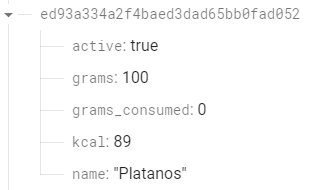
\includegraphics[width=0.5\textwidth]{Images/Capitulo5/alimentsTable.png}
    \caption{Entrada de la colección de documentos de alimentos}
    \label{fig:tabla_aliments}
\end{figure}


%%%%%%%%%%%%%%%%%%%%%
%%%TABLA DE COMENTARIOS%%%
%%%%%%%%%%%%%%%%%%%%%

\subsection{Colección de documentos de comentarios}
Esta colección de documentos contiene la información de cada comentario registrado en la aplicación (ver figura \ref{fig:tabla_comentarios}).

Concretamente contiene una lista de identificadores de dietas que tienen al menos un comentario.
Cada identificador de dieta, contiene dentro una lista de identificadores de comentarios. Dentro de cada identificador de comentario, se encuentran los siguientes campos:

\begin{itemize}
\item \textbf{Identificador de la dieta}
    \begin{itemize}
        \item \textbf{Identificador del comentario} generado automáticamente por Firebase.
        \begin{itemize}
            \item \textbf{Comment}: campo que contiene el comentario que ha escrito el usuario.
            \item \textbf{Date}: la fecha y hora a la que se escribió el comentario.
            \item \textbf{User}: el identificador del usuario que ha escrito el comentario.
        \end{itemize}
    \end{itemize}
\end{itemize}

%FOTO DE LA TABLA%
\begin{figure}[H]
    \centering
    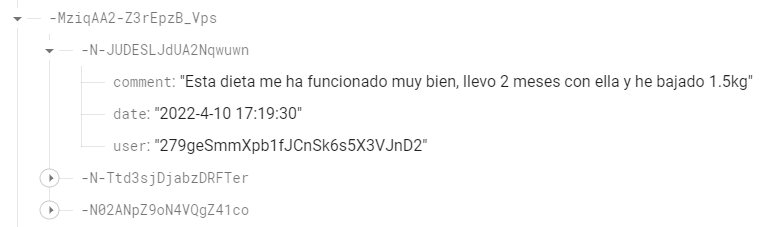
\includegraphics[width=0.9\textwidth]{Images/Capitulo5/tabla_comentarios.png}
    \caption{Entrada de la colección de documentos de comentarios}
    \label{fig:tabla_comentarios}
\end{figure}



%%%%%%%%%%%%%%%%%%%%%
%%%TABLA DE PASOS%%%
%%%%%%%%%%%%%%%%%%%%%

\subsection{Colección de documentos de pasos}
Esta colección de documentos contiene la información de los pasos realizados por cada usuario registrado en la aplicación (ver figura \ref{fig:tabla_pasos}).

Concretamente contiene una lista de identificadores únicos de cada usuario. Cada identificador tiene asociado un hashmap  de pares clave valor, donde la clave es la fecha y el valor son los pasos que ha hecho el usuario ese día. El propio funcionamiento de claves de Firebase hace que las fechas insertadas se ordenen cronológicamente. La estructura de una entrada en la colección de documentos es la siguiente:

\begin{itemize}
    \item \textbf{Identificador del usuario}
    \begin{itemize}
        \item \textbf{Fecha} en la que se registraron los pasos - \textbf{Nº de pasos} caminados durante ese día.
    \end{itemize}
\end{itemize}

\begin{figure}[H]
    \centering
    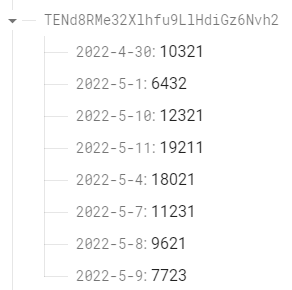
\includegraphics[width=0.5\textwidth]{Images/Capitulo5/stepsTable.png}
    \caption{Entrada de la colección de documentos de pasos}
    \label{fig:tabla_pasos}
\end{figure}

%%%%%%%%%%%%%%%%%%%%%
%%%TABLA DE PESOS%%%
%%%%%%%%%%%%%%%%%%%%%

\subsection{Colección de documentos de pesos}
Esta colección de documentos contiene la información del peso de cada usuario registrado en la aplicación (ver figura \ref{fig:tabla_pesos}).

Concretamente contiene una lista de identificadores únicos de cada usuario. Cada identificador tiene asociado un hashmap de pares clave valor, donde la clave es la fecha y el valor es el peso que el usuario ha registrado ese día. El propio funcionamiento de claves de Firebase hace que las fechas insertadas se ordenen cronológicamente.

La estructura de una entrada en la colección de documentos es la siguiente:

\begin{itemize}
    \item \textbf{Identificador del usuario}
    \begin{itemize}
        \item \textbf{Fecha} en la que se registró el peso - \textbf{Peso} del día indicado 
    \end{itemize}
\end{itemize}

\begin{figure}[H]
    \centering
    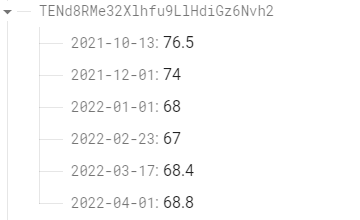
\includegraphics[width=0.5\textwidth]{Images/Capitulo5/tabla_pesos.png}
    \caption{Entrada de la colección de documentos de pesos}
    \label{fig:tabla_pesos}
\end{figure}

%%%%%%%%%%%%%%%%%%%%%
%%%TABLA DE HISTORIAL DE DIETAS%%%
%%%%%%%%%%%%%%%%%%%%%

\subsection{Colección de documentos de historial de dietas}
Esta colección de documentos contiene la información sobre las distintas dietas que ha seguido el usuario (ver figura \ref{fig:diet_history_table}).

La colección de documentos de historial de dietas contiene una lista de identificadores únicos de cada usuario. Cada uno de ellos tiene a su vez, una lista de los identificadores de al menos una las dietas que ha seguido. Cada dieta posee una entrada que indica la fecha en la que se consumió el alimento y, por cada una de estas fechas, se almacena la cantidad del alimento consumido.

\begin{itemize}
    \item \textbf{Identificador del usuario}
    \begin{itemize}
        \item \textbf{Identificador de la dieta} 
        \begin{itemize}
            \item \textbf{Fecha} en la que se consumió el alimento
              \begin{itemize}
                \item \textbf{Identificador del alimento} - \textbf{Cantidad de alimento} consumido en esa fecha
              \end{itemize} 
        \end{itemize}
    \end{itemize}    
\end{itemize}


\begin{figure}[H]
    \centering
    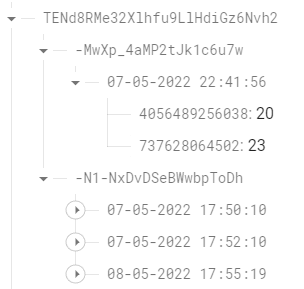
\includegraphics[width=0.5\textwidth]{Images/Capitulo5/dietHistoryTable.png}
    \caption{Entrada de la colección de documentos historial de dietas}
    \label{fig:diet_history_table}
\end{figure}


%%%%%%%%%%%%%%%%%%%%%
%%%ALMACENAMIENTO DE ARCHIVO%%%
%%%%%%%%%%%%%%%%%%%%%
\section{Almacenamiento de archivos}
Para el almacenamiento de archivos e imágenes se utiliza Firebase Storage, los datos que almacena son las imágenes de los usuarios y los documentos con extensión ``\texttt{.pdf}`` que se pueden añadir a una dieta.

La estructura que usa Firebase Storage es un sistema de directorios que tiene la siguiente forma:
\begin{itemize}
    \item \textbf{DietNow}
    \begin{itemize}
        \item \textbf{diets}: carpeta donde se almacenan todos los documentos asociados a las dietas.
            \begin{itemize}
                \item Identificador de la dieta: carpeta donde se almacenan los documentos de dicha dieta.
                \begin{itemize}
                    \item Nombre del documento pdf: hash \texttt{MD5} del documento.
                \end{itemize} 
            \end{itemize}
        \item \textbf{images}:   
            \begin{itemize}
                \item Imagen de perfil del usuario: para identificar cada imagen de usuario, éstas se suben con la estructura ``\texttt{profile\_\textbf{<identificador del usuario>}.jpg}``.
            \end{itemize}
    \end{itemize}
\end{itemize}

A continuación, en las figuras \ref{fig:storage_diet} y \ref{fig:storage_user}, se muestra una vista detallada en Firebase Storage de un documentos asociado a una dieta y la imagen de perfil de un usuario, respectivamente.

\begin{figure}[H]
    \centering
    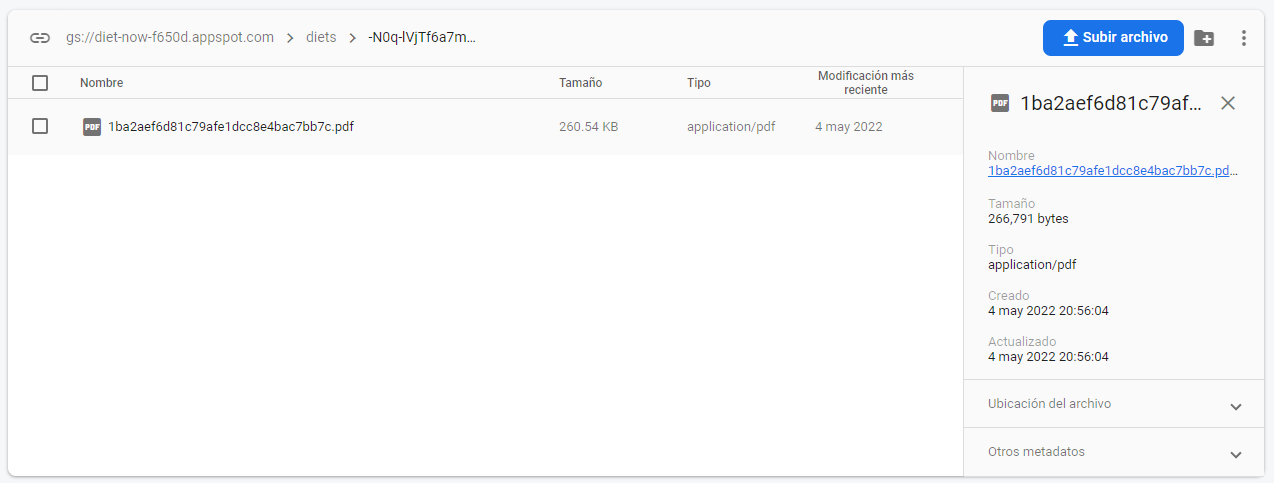
\includegraphics[width=\textwidth]{Images/Capitulo5/dietPdf.png}
    \caption{Vista detallada de un documento de una dieta}
    \label{fig:storage_diet}
\end{figure}

\begin{figure}[H]
    \centering
    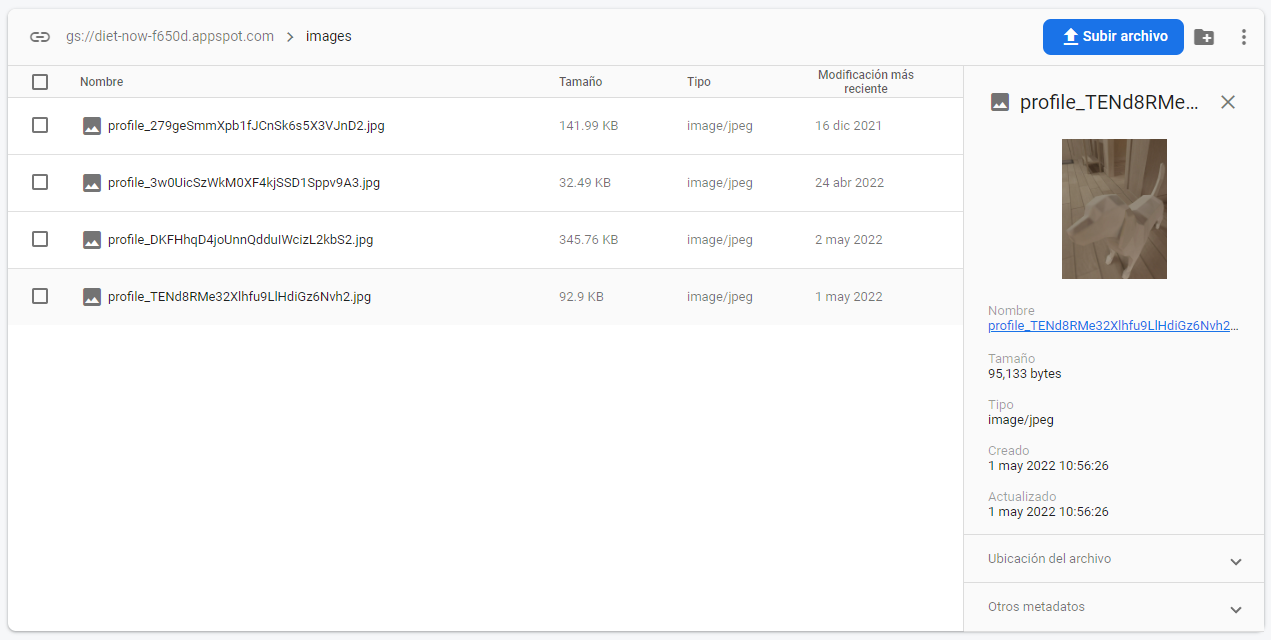
\includegraphics[width=\textwidth]{Images/Capitulo5/userImage.png}
    \caption{Vista detallada de la imagen de perfil de un usuario}
    \label{fig:storage_user}
\end{figure}